\documentclass[11pt, oneside]{article} 
\usepackage{geometry}
\geometry{letterpaper} 
\usepackage{graphicx}
	
\usepackage{amssymb}
\usepackage{amsmath}
\usepackage{parskip}
\usepackage{color}
\usepackage{hyperref}

\graphicspath{{/Users/telliott_admin/Tex/png/}}
% \begin{center} 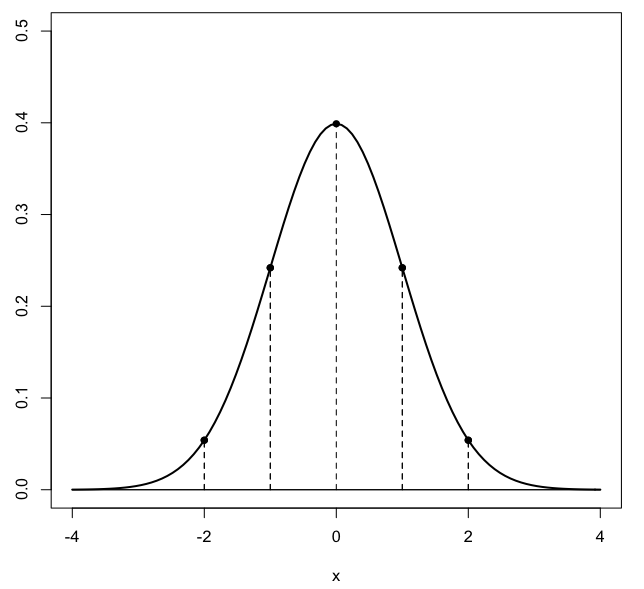
\includegraphics [scale=0.4] {gauss3.png} \end{center}

\title{Hatbox Theorem}
\date{}

\begin{document}
\maketitle
\Large

A famous result of Archimedes, among many others, is called the hat-box theorem, which states that the surface area of a sphere is equal to the lateral surface area of a cylinder which just encloses it, as we had above.  (Lateral area does not count the end pieces).

For a sphere and cylinder of radius $R$, the cylinder has surface area  of the circumference $2 \pi R$ times the height $2R$ for a total of $4 \pi R^2$.

Archimedes showed that this is true not just for the whole, but for any slice or section through the sphere.  That's pretty amazing.
\begin{center} 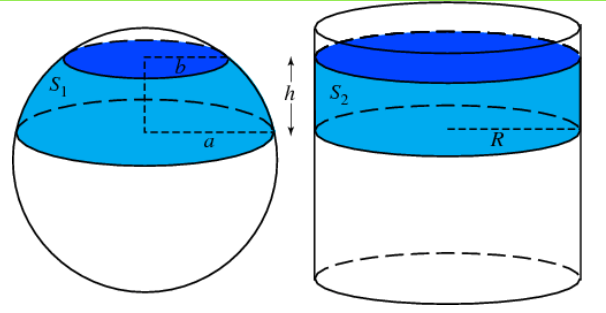
\includegraphics [scale=0.4] {hat_box_thm.png} \end{center}

Let's sketch a geometric proof briefly.  

First, consider a thin strip of surface area extending around the sphere on a great circle (such as the equator). The surface area will be the circumference times the width of the belt, or $2 \pi R \times h$.

Second, this is true even for a belt that is not at the equator.  Consider this figure:
\begin{center} 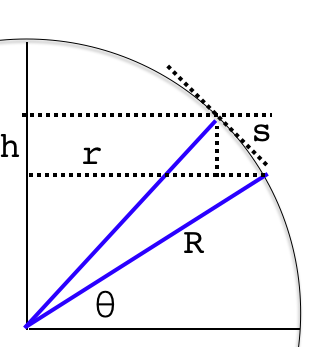
\includegraphics [scale=0.4] {slant_height.png} \end{center}

What is the surface area contained between two horizontal cuts of the sphere along the dotted lines?  Such a strip is called a "spherical belt".  If the slice is very thin, then the circumference at the top and bottom of the slice will be approximately the same, with radius $r = R \cos \theta$.

To get the surface area, we must multiply the circumference $2 \pi r$ by the width of the belt.  The width is not the height $h$ but $s$ (called the slant height), because of the tilt of the surface.

For a very thin slice, the angle $\theta$ won't change much in going from the first blue radius $R$ to the second one.  Seeing this, it is then not hard to work out that the angle between $s$ and $h$ in the right triangle containing them both is equal to $\theta$ 

\begin{center} 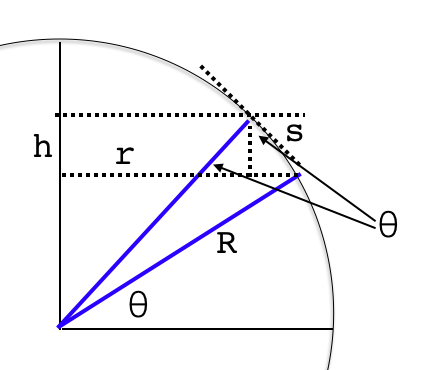
\includegraphics [scale=0.4] {slant_height2.png} \end{center}
so
\[ \cos \theta = \frac{h}{s} \]
The area is
\[ a = 2 \pi r s = 2 \pi R \cos \theta \frac{h}{\cos \theta} = 2 \pi R h \]
The same as before.

Third, consider the "belt" at the very top of the sphere.  This region is more of a "spherical cap", like a contact lens or one of the poles of earth.

We recall a famous result concerning chords of a circle.
\begin{center} 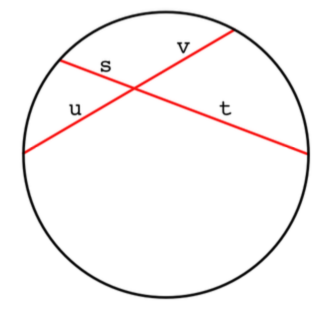
\includegraphics [scale=0.5] {stuv.png} \end{center}
\[ st = uv \]
This relationship holds for any two chords of the circle.  In particular, it holds for the chord consisting of $r + r$ and the chord consisting of $h + (2R - h)$.  
\begin{center} 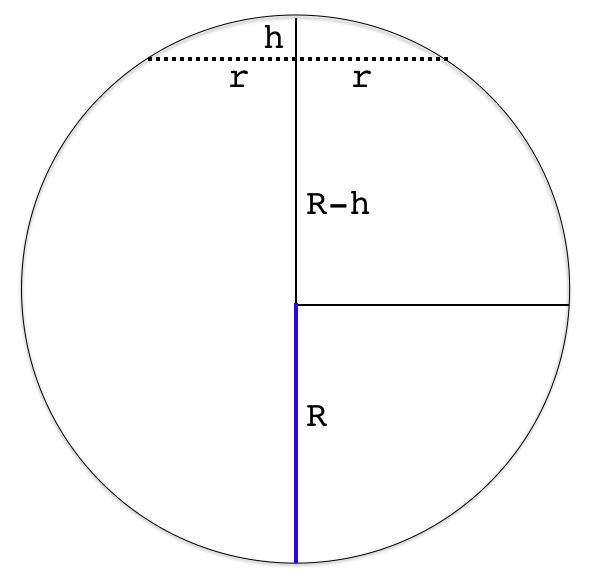
\includegraphics [scale=0.3] {2Rh.png} \end{center}

By the above theorem
\[ r^2 = h (2R-h) = 2Rh - h^2 \approx 2 Rh \]
Since $h$ is small, we can neglect a factor of $h^2$.

The area of the circle is 
\[ a = \pi r^2 = 2 \pi R h \]
so we have the same rule as above.

Therefore, for \emph{every} belt of height $h$, the area is $2 \pi R h$.

In summing up the contributions from each belt of width $h_i$
\[ A = \sum a = \sum 2 \pi R h_i = 2 \pi R \sum h_i  \]
But $\sum h_i$ is just equal to $R$ so we have
\[ A = 2 \pi R^2 \]

The surface area of a hemisphere of radius $R$ is twice the area of its great circle.  Thus, the total area of the sphere is $4 \pi R^2$.

\subsection*{geometric proof}
Here is a geometric proof that assumes we know the volume of the sphere is
\[ V = \frac{4}{3} \ \pi R^3 \]

\begin{center} 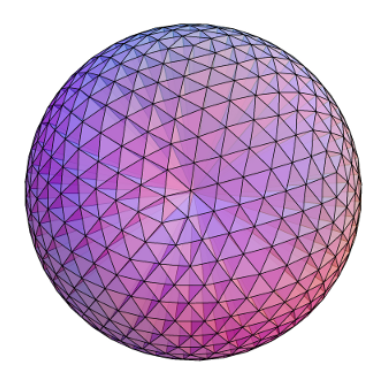
\includegraphics [scale=0.4] {sphere_area.png} \end{center}
Divide the whole sphere up into triangular prisms.  Each one has volume $dV = 1/3 \ R \ dA$.  So for the whole thing the volume =
\[ \frac{4}{3} \ \pi R^3 = \frac{1}{3} R \ A \]
\[ A = 4 \pi R^2 \]


\end{document}